\section{環境構築}
\subsection{ローカルでの環境構築}
\TeX でコンパイルを行うためには, TeX Liveをインストールする必要がある. 
本書執筆時点(\today 現在)では, TeX Live 2023が最新バージョンであるため, 
ここでは, TeX Live 2023のインストール方法を紹介する. 
\subsection{TeX Live 2023のインストール}
% Windowsでのインストール方法を簡単に述べる. 
% \begin{enumerate}
%   \item インターネットに置いてあるTeX Liveのインストールファイルをダウンロードする. 
%   \item TeX Liveをインストールする. 
%   \item Visual Studio Codeの拡張機能をインストールする. 
%   \item Visual Studio Codeの設定をしてVS CodeからTeXを使えるようにする. 
% \end{enumerate}
\subsubsection{Windowsの場合}
\url{https://mirror.ctan.org/systems/texlive/tlnet/install-tl-windows.exe}からインストールファイルをダウンロードする. 
ダウンロードが終わったら, エクスプローラを開き, \texttt{install-tl-windows.exe}を起動する. このとき, 
ファイル名を\textbf{右クリック}して「管理者として実行」をクリックすると, 全てのユーザ向けにインストールする
ことができるため, 必要に応じて管理者権限で実行すると良い. \\
exeファイルを実行すると, 次のようなウィンドウが立ち上がる. デフォルトでinstallが選ばれているので, 
installにチェックを入れたまま「Next >」をクリックする. 次のウィンドウでもそのまま「Install」を押せば, 
インストールが開始される. なお, この作業は非常に時間がかかるため, 注意が必要. 
\begin{figure}[htbp]
  \centering
  \begin{minipage}[b]{.49\textwidth}
    \centering
    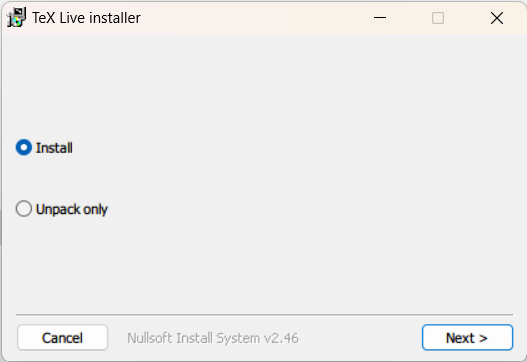
\includegraphics[width=\linewidth]{LTG_Resume_src/install_windows_1.png}
    \caption{インストールウィンドウ(Windows)(1)}
    \label{fig:ins_win_1}
  \end{minipage}%
  \hspace{.01\textwidth}
  \begin{minipage}[b]{.49\textwidth}
    \centering
    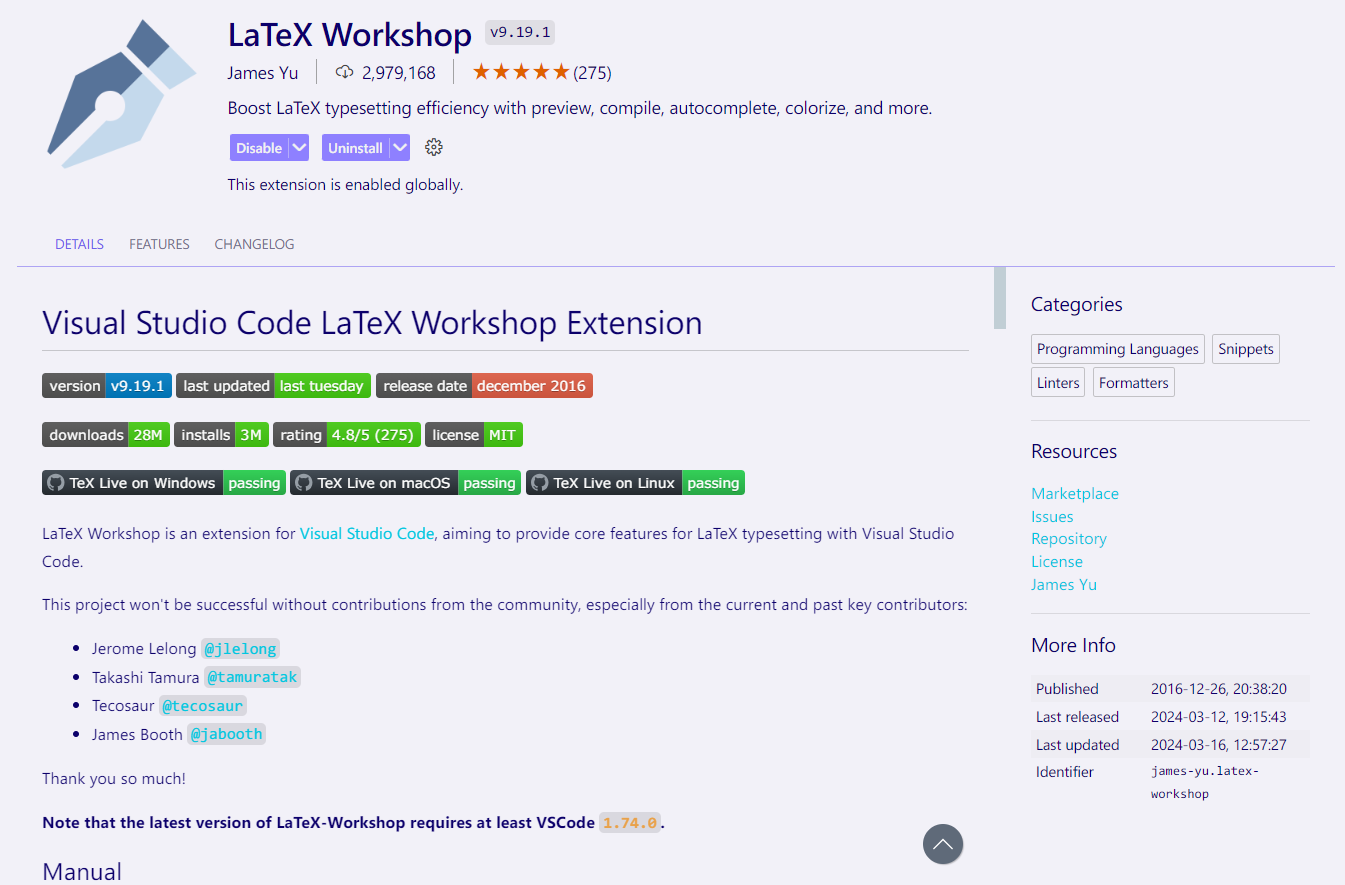
\includegraphics[width=\linewidth]{LTG_Resume_src/install_windows_2.png}
    \caption{LaTeX Workshop拡張機能}
    \label{fig:ins_win_2}
  \end{minipage}
\end{figure}

\subsection{VS CodeにTeXの拡張機能を追加する}
TeX Liveのインストールが終われば, 次はVS Codeから\TeX をコンパイルできるようにする
必要がある. まず, \TeX の拡張機能をインストールしよう. VS Codeの「拡張機能」にて, 
「LaTeX Workshop」と検索すれば同名の拡張機能が出てくるため, それをインストールする. 
(図\ref{fig:ins_win_2}参照)\\

基本的には以上で作業は完了である.